\section{System Overview}
\label{sec-system}

As state in former section, we build a ranking system for scholarly data analysis. Fig. \ref{fig:frame} shows the framework of our system, which consists of three main components, \itshape Storage, Query Engine \upshape and \itshape Visualizer \upshape respectively. And we demonstrate some scenarios that can be supported by our system.

\subsection{System Framework}
% The framework of the system consists of three main components, storage, query engine and visualizer.

\subsubsection{Storage}
\par
The component of storage consists of property graph and transaction. Heterogeneous academic data is stored as property graph model which possesses nodes and relationships, and we use transaction to ensure the predictability of relationship-based queries.

\par
We apply a popular graph database Neo4j \cite{Neo4j} to manage and operate massive scholarly data based on the following reasons. First, scholarly data is naturally structured data connected by the reference relationship. At the same time, graph database has great performance implementation handling connections. Second, Neo4j is provided with highly performant read and write scalability thanks to native graph storage and processing. Thus, it works well in managing scholarly data and searching subgraphs.

\par
In order to manage effectively and query efficiently with Neo4j, we design a graph schema mainly based on two principles. (1) Nodes for things and relationships for structure. (2) We take into consideration of the query ability of the graph schema and adopt specific trade-offs. Thus, we model academic data as a huge heterogeneous graph, shown in Fig. \ref{fig:schema}, which contains more than one billion nodes and over two billion relationships.

\begin{figure}
\centering
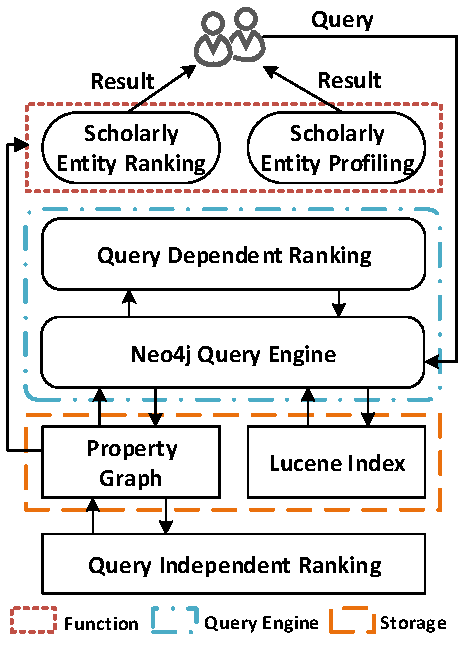
\includegraphics[width=\columnwidth]{systemFrame.pdf}
\caption{system framework}
\label{fig:frame}
\end{figure}


\begin{figure}
\centering
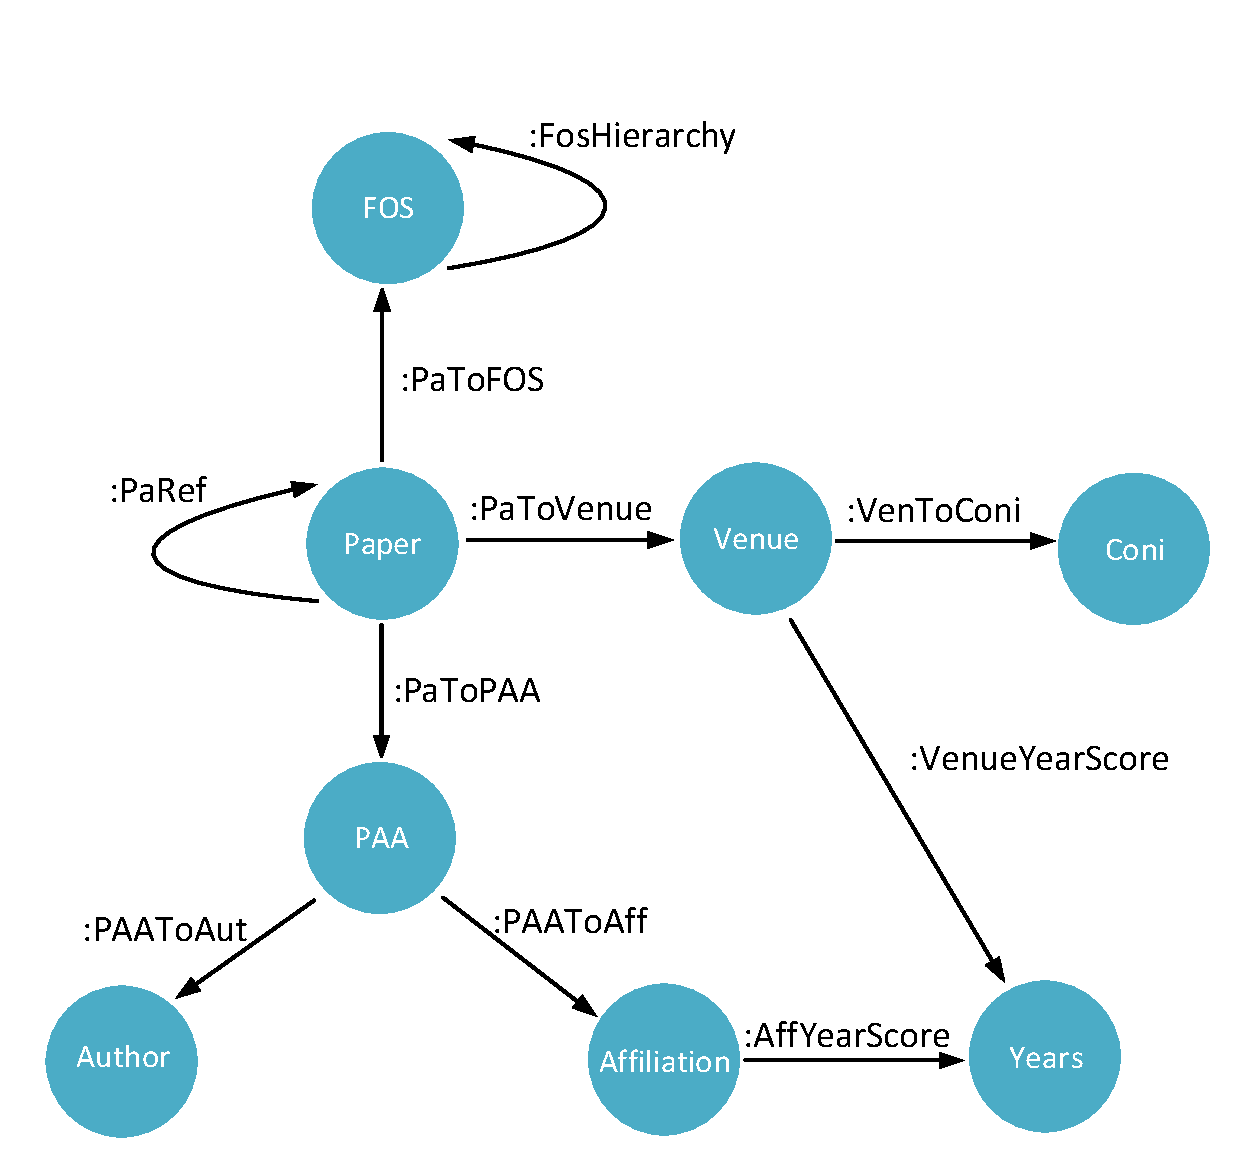
\includegraphics[width=\columnwidth]{neo4jSchema.pdf}
\caption{Neo4j schema design}
\label{fig:schema}
\end{figure}

\par
The graph schema contains seven type of entities: author, affiliation, field of study, paper, venue(journal and conferences \itshape e.g., \upshape KDD, ICDE ), conference instance (\itshape e.g., \upshape KDD 2019, ICDE 2019), years. In order to query efficiently, we introduce an additional node PAA to represent the paper-author-affiliation n-ary relationships. Intuitively, a paper get published in a journal/conference by the author means the edges among paper, author and venue node. 

\par
By employing ranking model as stated in section 2, we derive affiliation, author, venue and article ranking score using incremental computation \cite{ma2018query}. And those score is described as a property in the graph schema. In fact, we can apply any algorithms to rank scholarly entities in the graph schema.


\subsubsection{Query Engine}
Query engine is the main component that is responsible for handling scholarly data. It consists of lucene index, query optimizer, Neo4j query engine and ranking algorithm. Lucene index is especially important for retrieving articles from Neo4j. Obviously, we index article's title after using stop words, and index the distributed vector representation of words. 
\\ Lucene Index.
\\ why we need index. index is important for xxx 
\\ what we indexed?
\\ 1. title after using stop word in desk.
\\ 2. vector, word representation
\\ Query Optimizer and
\\ Neo4j Query Engine
\\ Ranking Algorithm
\\ relevance, ranking results.

\subsubsection{Visualizer}
visualization
\\ use interface
\\ search affiliation, author, venue, articles
\\ visualization for author, articles?




\subsection{System Demonstration}

demonstration graph


